\documentclass[main]{subfiles}

\begin{document}
	\begin{Proof}
		%ЗДЕСЬ ОЧЕНЬ МНОГО ОШИБОК TO-DO ИСПРАВИТЬ!!!
		%Выглядит очень плохо
		\[p = a\]
		\[f(p + h) = f(p) + \us{= 0}{d_p} f(h) + \frac{1}{2} d^2_p f(h) + \frac{1}{2}\alpha(h) \cdot \Abs{h}^2 \qq
			\alpha(h) \to 0\]
		\[2(f(p + h) - f(p)) = d_p^2 f (h) + \alpha(h) \cdot \Abs{h}^2\]
		\[d^2_p f \text{ на } S = \{h : \Abs{h} = 1\}\]
		Случай 1:
		\[\letus \ \us{\text{непр. как ф. от h}}{d_p^2 f(h)} > 0 \q \forall h \neq 0\]
		\[m = \min_{h \in S} d_p^2 f(h) = d^2_p f(\xi) \q \xi \in S\]
		\[M = \max_{h \in S} d_p^2 f(h) = d^2_p f(\mu) \q \mu \in S\]
		\[d^2_p f(h) = \sum^n_{i, j= 1} (\frac{\partial^2 f}{\partial x_{i} \partial x_{j} }
			\frac{h_i}{\Abs{h}} \frac{h_j}{\Abs{h}}) \cdot \Abs{h}^2 = \Abs{h}^2 d^2_p f(\frac{h}{\Abs{h}}) \geq m \cdot \Abs{h} ^2\]
		\[\text{Т.к. } \alpha(h) \to 0, \text{ то:}\]
		\[\exists \delta > 0 : \forall \Abs{h} < \delta \q \abs{\alpha(h)} < \frac{m}{2}\]
		\begin{multline*}
		    2(f(p + h) - f(p)) = d_p^2 f(h) + \alpha(h) \Abs{h}^2 = \\ = \Abs{h}^2 \Br{\ub{\geq m}{d_p^2 f \Br{\frac{h}{\Abs{h}}}} +
			\alpha(h)} \geq \frac{m}{2} \cdot \Abs{h}^2 > 0 \q \forall h \neq 0
		\end{multline*}
		\[\abs{\alpha} < \frac{m}{2}, \text{ т.е } f(p + h) > f(p)\q \forall \Abs{h} < \delta\]
		т. о. $p$ --- т. стр. лок. $\min$\\
		Случай 2: Аналогично\\
		Случай 3:
		\[\displaystyle \letus m = \min_{\Abs{h} = 1} d_p^2 f(h) = d_p^2 f(\xi) < 0\]
		\[M = \max_{\Abs{h} = 1} d_p^2 f(h) = d_p^2 f(\mu) > 0 \]
		\[? \exists t :  f(p + t \xi) < f(p)\]
		\[f(p + t \mu) > f(p)\]
		\[f(p + \us{h}{t \cdot \xi}) - f(p) = t^2 (d^2_p f(\xi) + \alpha(h)) \]
		\[\exists \delta > 0 : \Abs{h} < \delta \Ra \abs{\alpha(h)} < \frac{m}{2}\]
		\[\Ra \abs{t} < \delta \q f(p + t\xi) - f(p) < 0 \q \forall t \neq 0\]
		Аналогично $\exists \widetilde{\delta} : \Abs{h} < \widetilde{\delta} \Ra
			\abs{\alpha(h)} < \frac{M}{2}$
		\[f(p + t\mu) - f(p) > 0 \q \forall h \neq 0\]
	\end{Proof}

	\begin{Example}
		\[f(x, y) = xy + \frac{1}{x} + \frac{1}{y} \qq x > 0 \q y > 0\]
		\[(x, y) = (1, 1) \text{ --- крит. точка}\]
		\[\begin{cases}
				f'_x = y - \frac{1}{x^2} = 0 \\
				f'_y = x - \frac{1}{y^2} = 0
			\end{cases}\]
		\[f''_{xx} = \frac{2}{x^3} \qq f''_{xy}  = 1 \qq f''_{yy} = \frac{2}{y^3}\]
		\[d^2_{(1, 1)} f(h) = (h_1, h_2) \begin{pmatrix}
				2 & 1 \\
				1 & 2
			\end{pmatrix}
			\begin{pmatrix}
				h_1 \\
				h_2
			\end{pmatrix}
			= 2 h_1^2 + 2h_1 h_2 + 2 h_2^2\]
		\[d^2_{(1,1)} f(h) > 0 \q \forall h \neq 0 \]
		т. о. $(1, 1)$ --- т. лок. $\min$
		%Я не из тех, кто чтит попов
		%Кто безотчетно верит в бога
	\end{Example}

	\newpage
	\subsection{Теорема об обратном отображении, доказательство леммы об операторе, близком к обратному}
		%самой теоремы тут нет
		\[A \text{ - лин. отобр.} \q A \in \LL(\R^n, \R^m)\]
		\[\text{Если $A$ --- обратимое отобр. $\Ra$ ?}\]
		\[m = n \q \ker A = 0\]
		\[\det A \neq 0  \q A(\R^n) = \R^n\]
		\[f : U \to \R^m \qq U \subset \R^n \text{ предпол., что } f \text{ --- диф. на }U\]
		\[f \text{ --- обратимо и } f^{-1} \text{ --- тоже диф-мо} \q f^{-1} : f(U) \to U  \]
		\[(f^{-1} \circ f)(x) = x \]
		\[d_x (f^{-1} \circ f) = d_{f(x)} f^{-1} \us{A}{d_x} f = E_n = \begin{pmatrix}
				1 & ...    & 0 \\
				0 & \ddots & 0 \\
				0 & ...    & 1
			\end{pmatrix} \RA n = m\]
		\[f : \us{\subset \R^n}{U} \to \R^n\]

    %кто прочитал это тот здохнет
	\begin{Theorem} [об обратном отображении]
		\[ \letus\ \us{\text{откр}}{U} \subset \R^n \q f \in C^1 (U) \q a \in U,\q d_a f \text{ --- обратим}\]
		Тогда $\exists U_a \subset U \text{ (окр. т. $a$):}$
		\begin{enumerate}
			\item $f \big|_{U_a}$ --- инъекция
			\item $f(U_a)$ --- откр.
			\item $f^{-1} \in C^1 \q (V= f(U_a) \to U_a)$
			\item $d_{f(a)} f^{-1} \circ d_a f = E_n$
		\end{enumerate}
	\end{Theorem}

	\begin{Example} \
		\begin{figure}[h!]
			\center{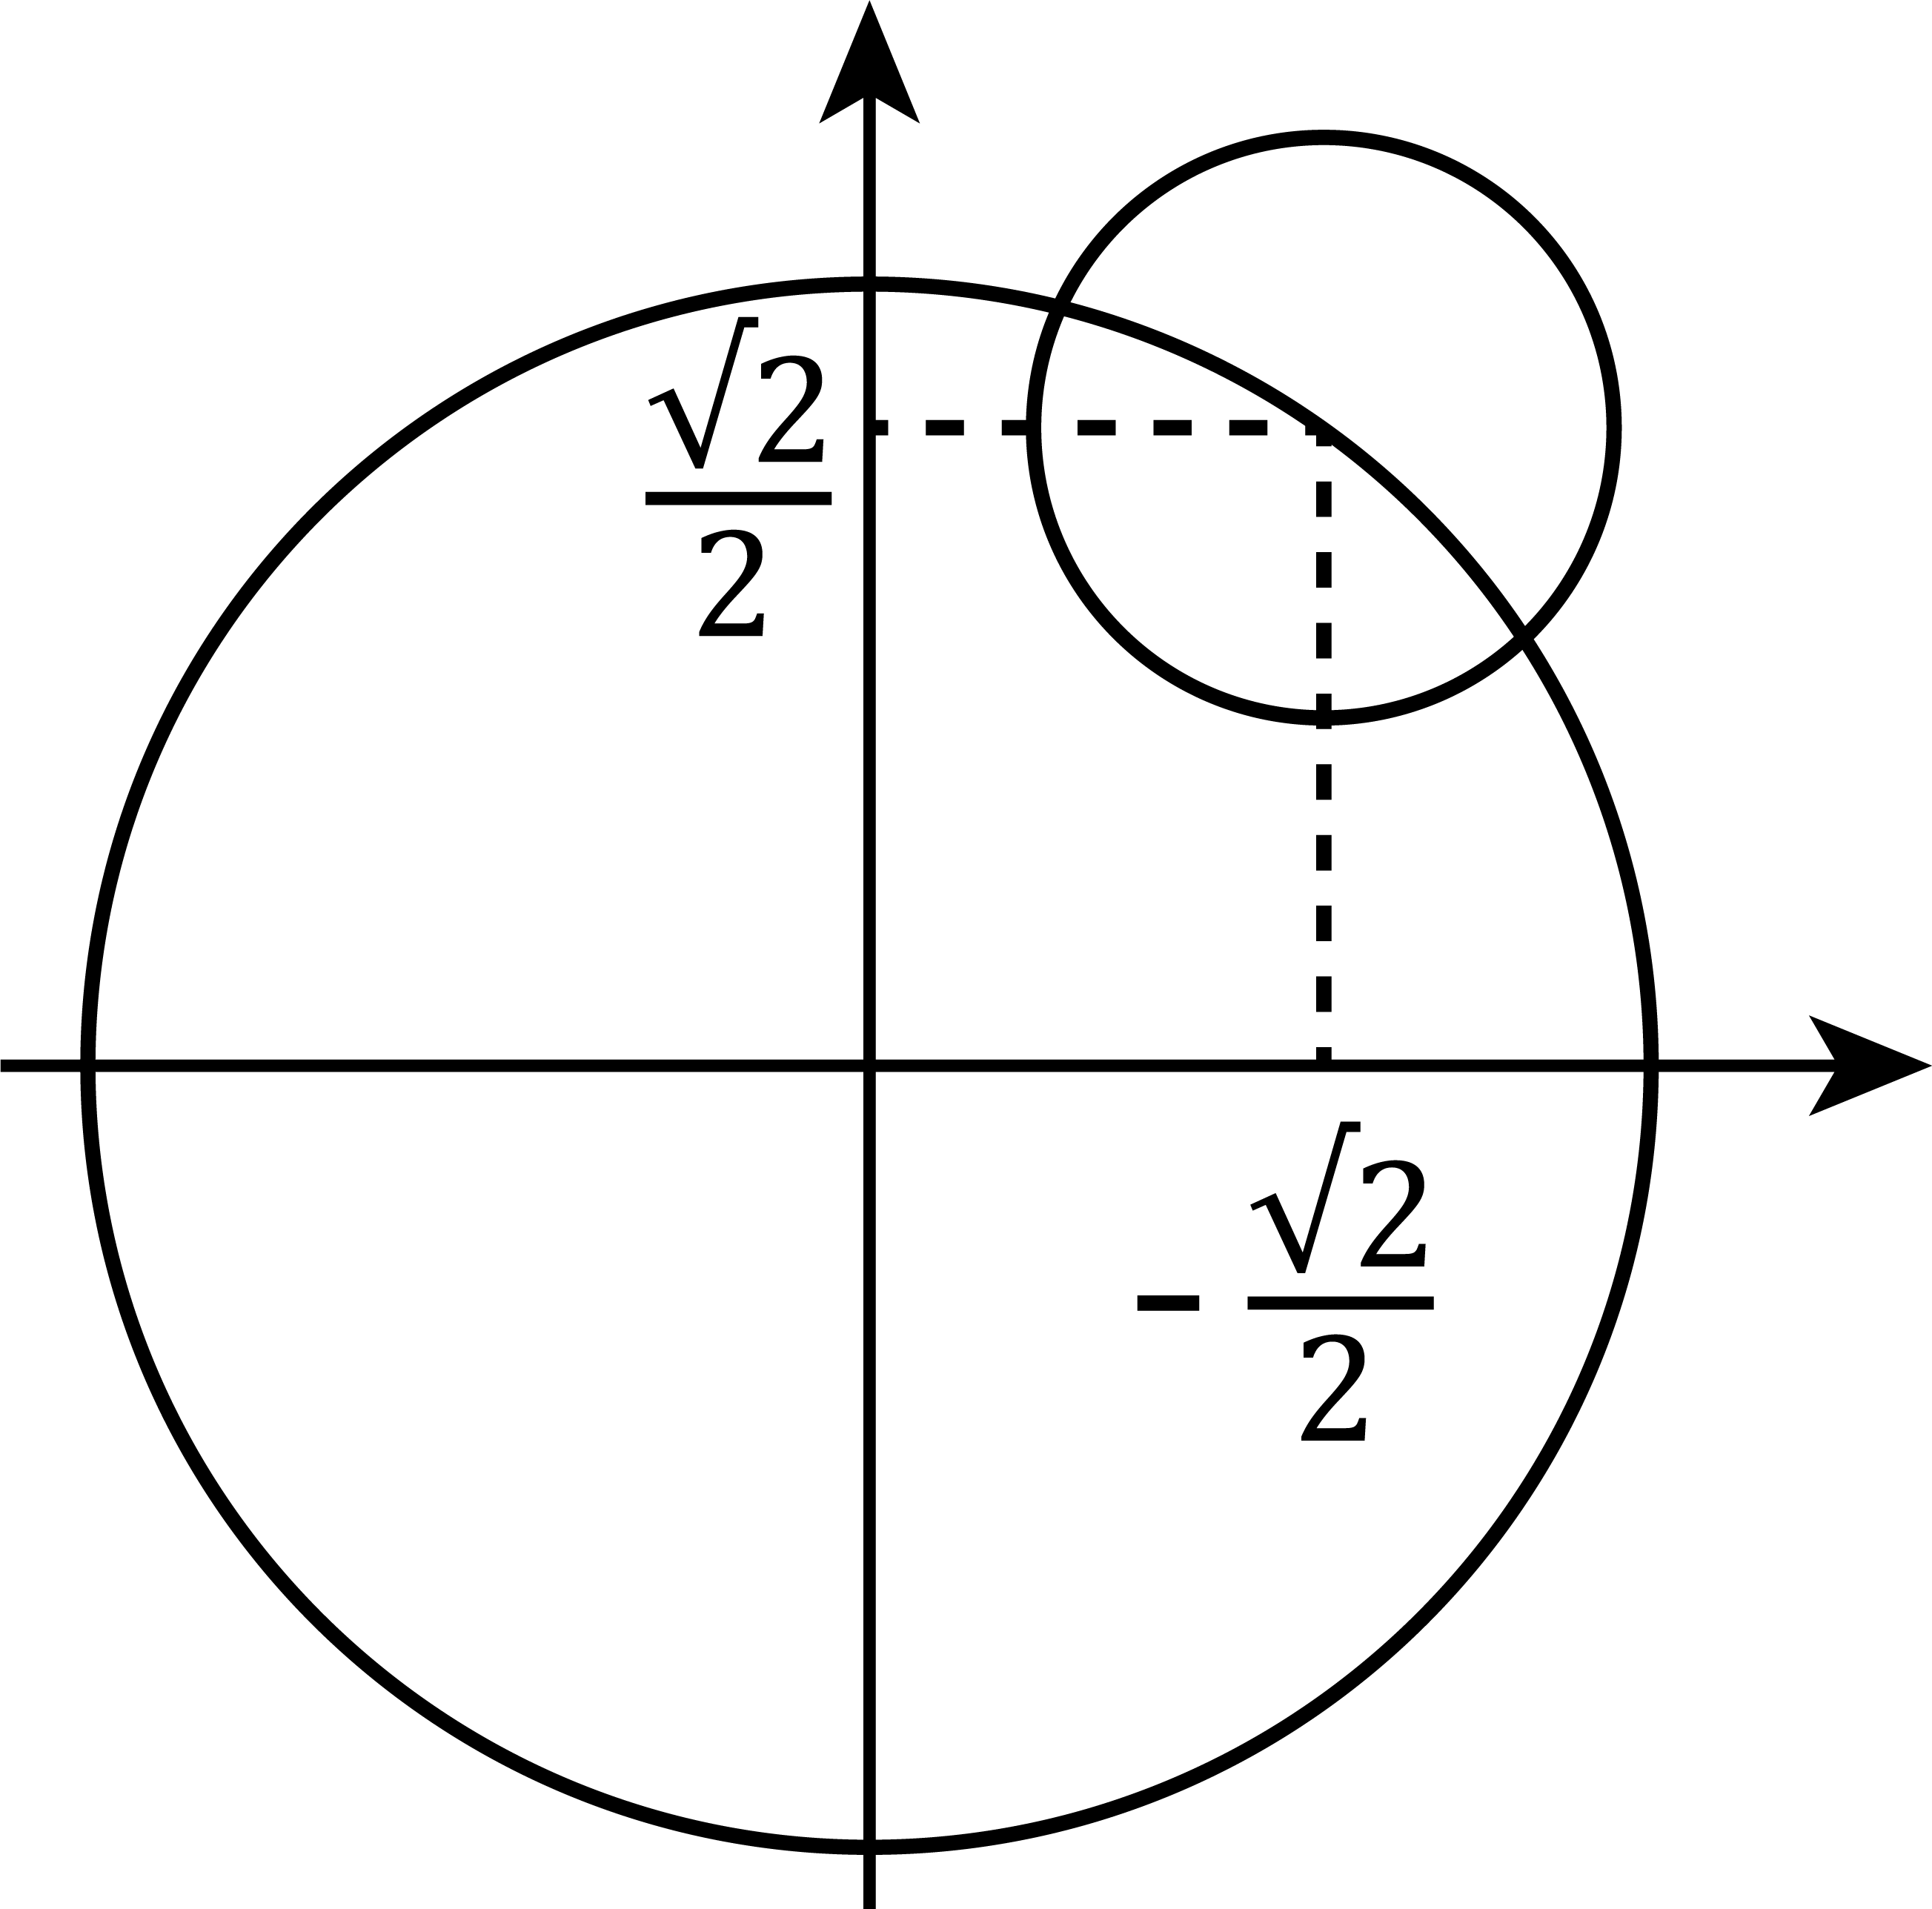
\includegraphics[width = 3cm]{pics/6_1}}
		\end{figure}
		\[n = 1\]
		\[f(x) = x^2\]
		\[a = -2\]
		\[d_af(h) = 2a \cdot h = -4h \text{ --- обратим}\]
		\[(d_0 f(h) = 0 \cdot h = 0 \text{ --- необр.})\]
		\[\exists U_a = (-3; -1) : f^{-1}(y) = - \sqrt{y} \]
	\end{Example}

	\begin{Lemma} [1, лемма об операторе, близком к обратимому]
		\[GL(n) \text{ --- группа обратимых операторов}\]
		\[\letus\ A \in GL(n)б\q B \in \LL(\R^n)\]
		\[\Abs{B - A} < \frac{1}{\Abs{A^{-1}}}\]
		Тогда:
		\begin{enumerate}
			\item $B \in GL(n)$
			\item Отобр. $A \to A^{-1}$ --- непр. (в операторной норме)
		\end{enumerate}
	\end{Lemma}

	\begin{proof}
		\begin{enumerate}
			\item $\alpha = \Abs{A^{-1}} \q \beta = \Abs{B - A}$
				\[\Abs{Ax} = \Abs{(A + B - B)x} \leq \Abs{Bx} + \Abs{(A - B)x}\]
				\[\Abs{Bx} \geq \Abs{Ax} - \Abs{(A-B)x}\]
				\[\Abs{x} = \Abs{A^{-1}Ax} \leq \us{\text{норма оп.}}{\Abs{A^{-1}}} \us{\text{норма вект.}}{\Abs{Ax}}
					\Ra \Abs{Ax} \geq \frac{1}{\alpha} \Abs{x}\]
				\[\Abs{Bx} \geq \Abs{Ax} - \Abs{(A - B)x} \geq \frac{1}{\alpha} \Abs{x} - \beta \Abs{x}
					= \Br{\frac{1}{\alpha} - \beta} \Abs{x} \q (*)\]
				\[\Abs{Bx} > 0\]
				\[\text{т.е. инъекция} \Ra B \in GL(n)\]
			\item $\Abs{A^{-1} - B^{-1}}$
				\[A^{-1} - B^{-1} = A^{-1}(B - A)B^{-1}\]
				\[\Abs{A^{-1} - B^{-1}} \leq \Abs{A^{-1}} \cdot \Abs{B - A} \cdot \Abs{B^{-1}}\]
				\[\text{Из (1) } \Ra \Abs{Bx} \geq (\alpha^{-1} - \beta) \cdot \Abs{\us{=B^{-1}(y)}{x}}\]
				\[\Abs{y} \geq \Br{\frac{1}{\alpha} - \beta} \Abs{B^{-1} y }\]
				\[\Abs{B^{-1}y } \leq \frac{\Abs{y}}{a - \beta} \qq \frac{1}{\alpha} = a\]
				\[\Abs{B^{-1}} \leq \frac{1}{a - \beta} \]
				\[\Abs{A^{-1} - B^{-1}} \leq \frac{1}{a} \cdot \beta \cdot \frac{1}{a - \beta}\]
				\[\Phi(A) = A^{-1}\]
				\[\Phi \text{ - непр в т. }A\]
				\[\forall \mathcal{E} > 0\ \exists \delta > 0 : \forall B : \Abs{B - A} < \delta \RA
					\Abs{A^{-1} - B^{-1}} \leq \frac{1}{a} \frac{\beta}{(a - \beta)} < \mathcal{E}\]
				\[a \text{ --- фиксир.}\]
				\[\beta \to 0\]
		\end{enumerate}
	\end{proof}

	\newpage
	\subsection{Теорема об обратном отображении, доказательство леммы об оценке приращения}

	\begin{Lemma} [2, лемма об оценке приращения]
		\[U \subset \R^n,\q f: U \to \R^m, \q f \text{ --- диф. на } U,\q \letus\ [a, b] \subset U\]
		\[\text{Тогда } \exists\ \Theta \in (0, 1) : c = a + \Theta(b-a),\text{ такая что:}\]
		\[\Abs{f(b) - f(a)} \leq \Abs{d_c f} \cdot \Abs{b - a}\]
		\begin{figure}[h!]
			\center{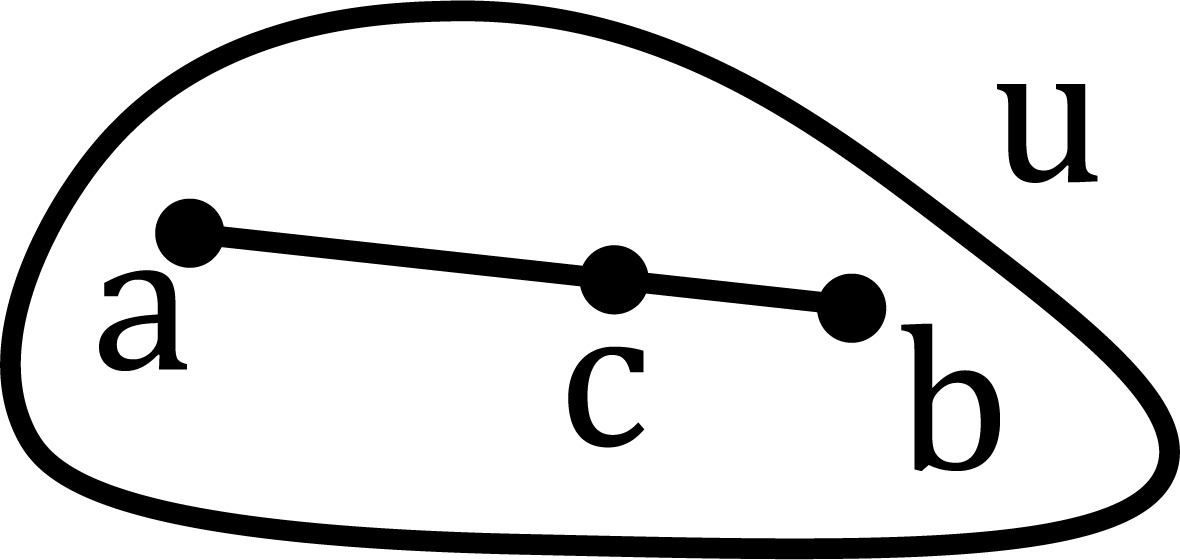
\includegraphics[width = 3cm]{pics/6_2}}
		\end{figure}
	\end{Lemma}

	\begin{Proof}
		\[\varphi(t) = (f(a + t(b - a));\ f(b) - f(a)) \text{ --- скал. произв в } \R^n\]
		\[t \in [0, 1] \q \varphi : [0, 1] \to \R\]
		Т. Лагранжа для функции $\varphi$
		\[\exists\ \Theta \in (0, 1) : \]
		\[\varphi(1) - \varphi(0) = \varphi'(\Theta) \cdot (1 - 0) = \Abs{f(b) - f(a)}^2\]
		\[\abs{\varphi'(\Theta)} = \abs{ (d_c f(b - a);\ f(b) - f(a))} \os{\text{КБШ}}{\circlesign{\leq}} \]
		\[c = a + \Theta(b - a)\]
		\[\circlesign{\leq} \Abs{d_c f(b-a)} \cdot \Abs{f(b) - f(a)} \leq \Abs{d_c f} \cdot \Abs{b - a} \cdot
			\Abs{f(b) - f(a)}\]
		\[\Ra \Abs{f(b) - f(a)} \leq \Abs{d_c f} \cdot \Abs{b - a}\]
	\end{Proof}
	Договоримся использовать
	\[A = d_a f\]
	\[\lambda = \frac{1}{4 \Abs{A^{-1}}}\]

	\newpage
	\subsection{Теорема об открытом отображении}

	\begin{Lemma} [3]
		\[\text{Пусть }f \in C^{1}(U \to \R^n), \q \us{\text{откр.}}{U} \subset \R^n. \q a \in U,\q d_af \text{ --- обратим}\]
		Тогда $\exists U_a:$
		\begin{enumerate}
			\item $\forall x \in U_a \q d_xf $ --- обратим
			      %рисунок с окрестностью в множестве
			\item $\forall x, \ x + h \in U_a$
				\begin{enumerate}
					\item $\Abs{f(x+h) - f(x) - d_a f(h)} \leq 2 \lambda \Abs{h}$
					\item $\Abs{f(x + h) - f(x)} \geq 2 \lambda \Abs{h}$
				\end{enumerate}
		\end{enumerate}
	\end{Lemma}

	\begin{proof}
		\begin{enumerate}
			\item $\text{Т.к } f \in C^{1}(U) \rla df \text{ как отобр. из } U \text{ в } \LL(\R^n, \R^n) \text{ --- непр.}$
				\[\mathcal{E} = 2\lambda \RA \exists  B_a : \forall x \in B_a \q \Abs{d_a f - d_x f} < 2 \lambda\]
				По лемме об операторе близком к обратимому
				\[(A \text{ - обр. и } \Abs{A - B} \leq \frac{1}{\Abs{A^{-1} }} \RA B \text{ --- обр.})\]
				\[\Abs{d_a f - d_x f} < 2\lambda < 4 \lambda = \frac{1}{\Abs{A^{-1}}} \RA d_xf \text{ --- обратим}\]
			\item $F(u) = f(u) - d_a f(u)$ %опять рисунок шарика в области U
				\[\Abs{d_cF} = \Abs{d_cf - d_af} < 2\lambda \q \forall c \in B_a\]
			\begin{enumerate}
				\item $\Abs{f(x + h) - f(x) - d_af(h)} = \Abs{F(x + h) - F(x)} \os{\text{лемма 2}}{\leq}$
				\[\leq \Abs{d_{x+ \Theta h} F} \cdot \Abs{h} < 2 \lambda \Abs{h}\]
				\item $\Abs{h} = \Abs{A^{-1}Ah} \leq \Abs{A^{-1}} \cdot \Abs{A h}$
				\[\Abs{Ah} \geq \frac{\Abs{h}}{\Abs{A^{-1}}} = 4 \lambda \Abs{h}\]
				\[\Abs{Ah} \leq \Abs{f(x + h) - f(x) - Ah} + \Abs{f(x + h) - f(x)}\]
				%\[\Abs{f(x + h) - f(x)} \leq \Abs{f(x + h) - f(x) - d_af(h)} + \Abs{d_afh} \os{\text{из (a)}}{ \leq}\]
				\[\Abs{f(x + h) - f(x)} \geq \Abs{Ah} - \Abs{f(x + h) - f(x) - Ah} \geq\]
				\[\geq 4\lambda \Abs{h} - 2\lambda \Abs{h} = 2 \lambda \Abs{h}\]
			\end{enumerate}
		\end{enumerate}
	\end{proof}

	\begin{Reminder}[теорема об обратном отображении]
		\[ \letus\ \us{\text{откр}}{U} \subset \R^n \q f \in C^1 (U) \q a \in U,\q d_a f \text{ --- обратим.}\]
		Тогда $\exists U_a \subset U \text{ (окр. т. $a$):}$
		\begin{enumerate}
			\item $f \big|_{U_a}$ --- инъекция
			\item $f(U_a)$ --- откр. \q $V = f(U_a)$
			\item $f^{-1} \in C^1 \q (V \to U_a)$
			\item $d_{f(a)} f^{-1} \circ d_a f = E_n$
		\end{enumerate}
	\end{Reminder}

	\begin{proof} [теоремы об обратном отобр.]
		\begin{enumerate}
			\item $B_a \text{ --- из леммы 3} \qq U_a = B_a$\\
			Уже знаем, что $\forall x \in B_a \q \Abs{d_a f- d_x f} < 2\lambda$
			\[\text{Из леммы 3 } \Abs{f(x + h) - f(x)} \geq 2 \lambda \cdot \Abs{h} > 0 \q \forall h \neq 0\]
			\[\text{т.е. } f \text{ --- инъекция}\]
			\item Докажем, что $f(B_a)$ --- откр., $V = f(B_a)$
			\begin{figure}[h!]
				\center{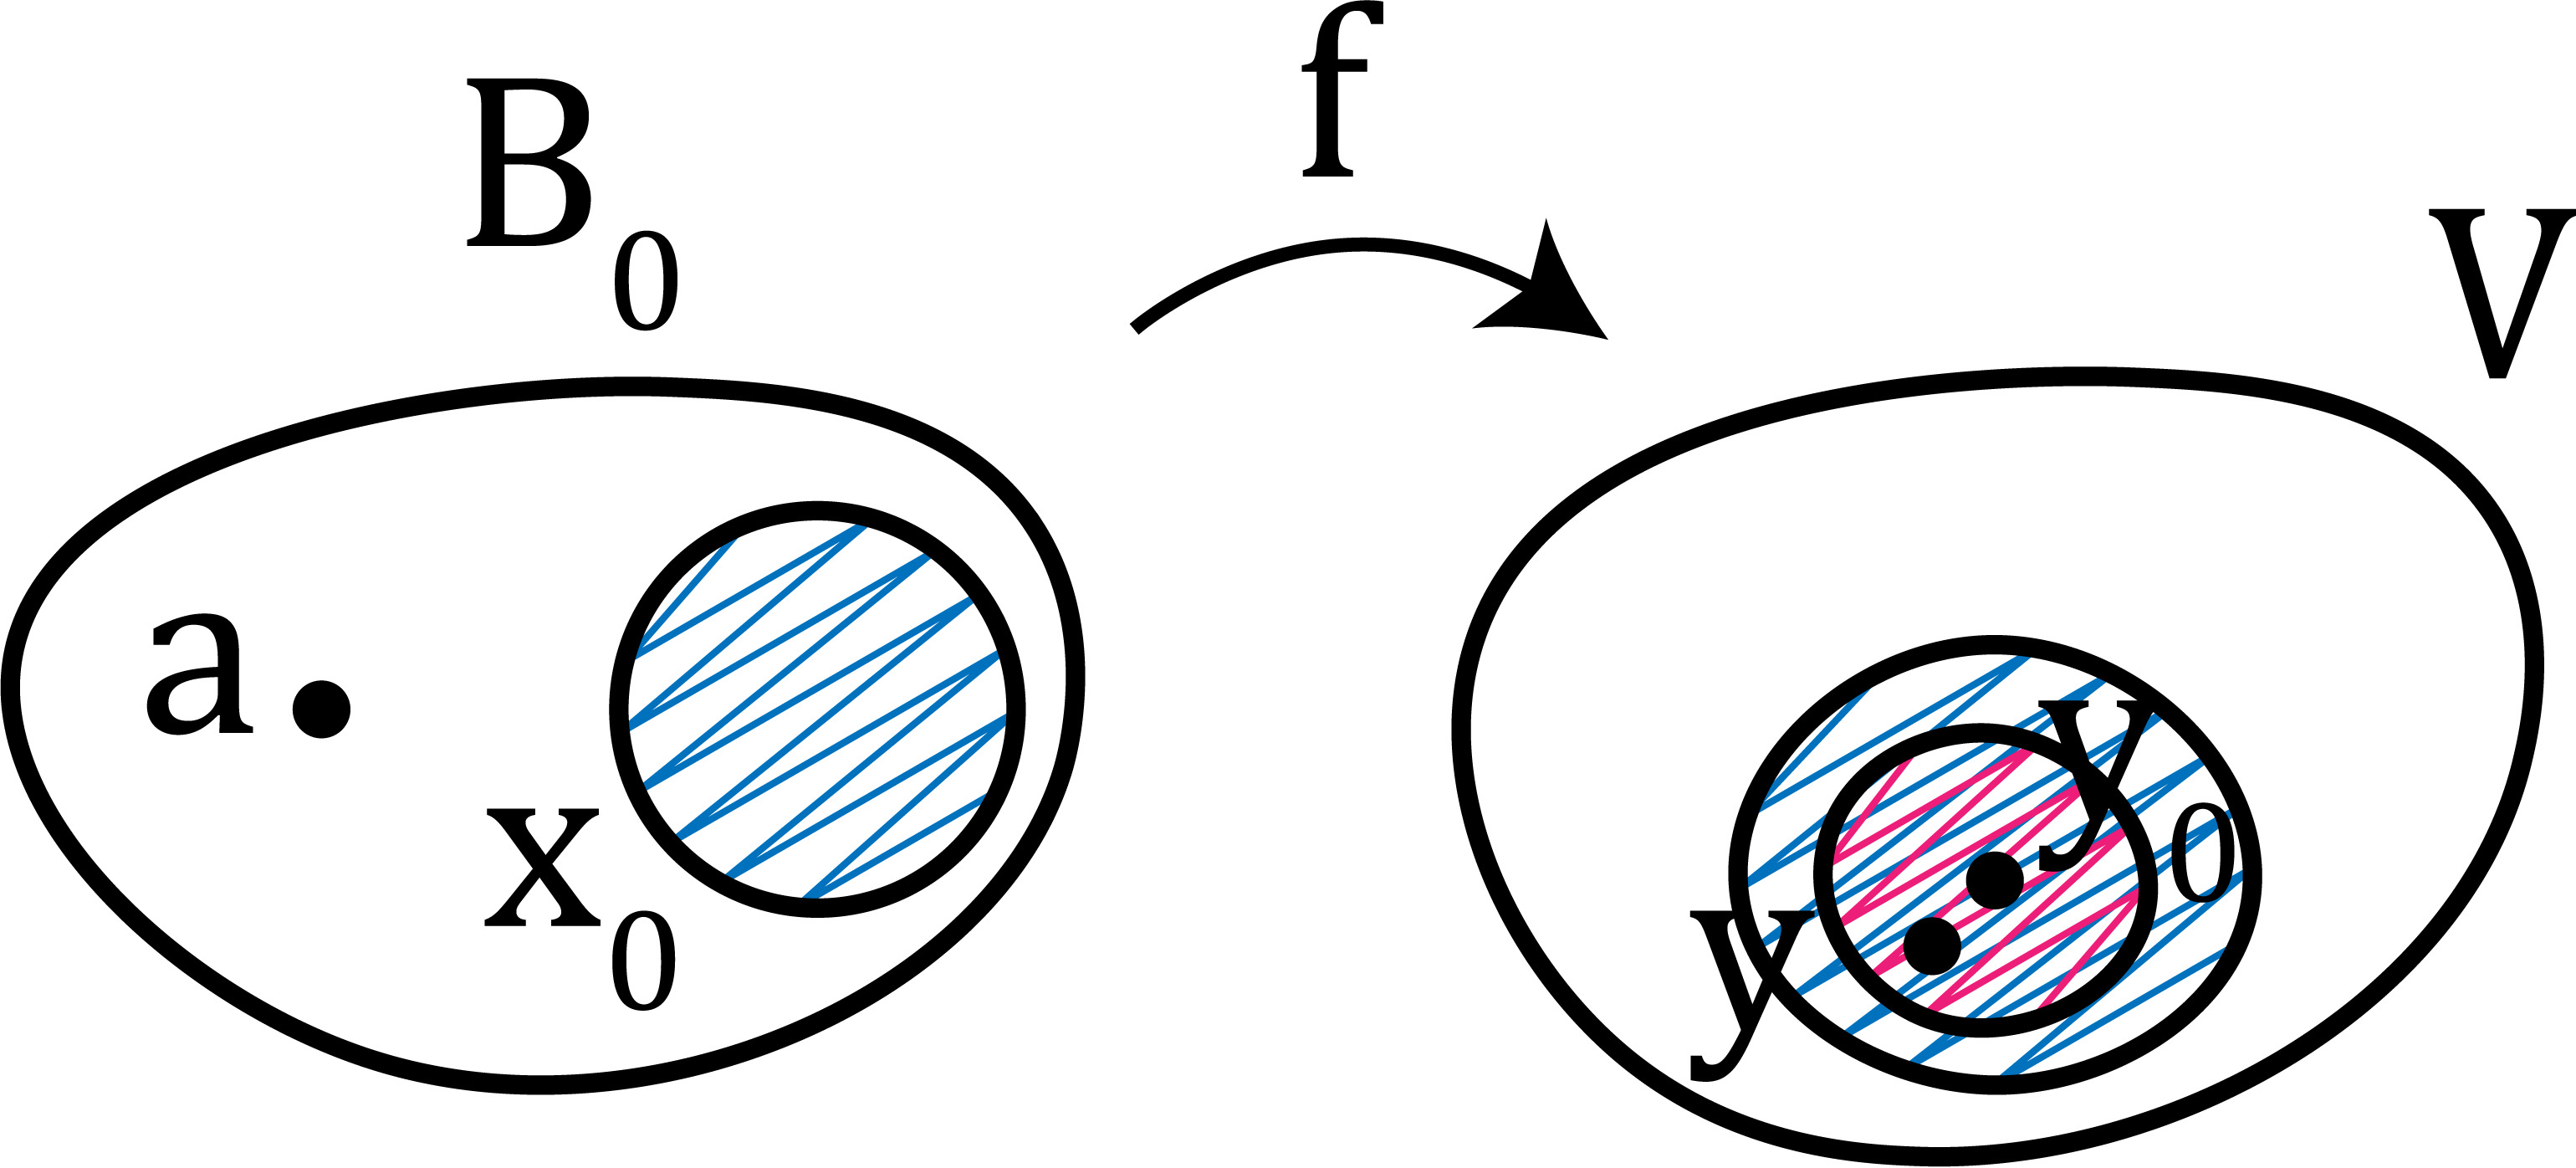
\includegraphics[width = 5cm]{pics/6_3}}
			\end{figure}
			\[\text{Зафиксируем } y_0 \in V: y_0 = f(x_0) \q x_o \in B_a\]
			\[\exists r > 0 : \q \ol{B(x_0, r)} \subset B_a \subset U\]
			\[\text{Цель: } B(y_0, \lambda_r) \subset f(B(x_0, r))\]
			\[\text{Рассмотрим } y \in B(y_0, \lambda_r)\]
			\[\Phi(x) = \Abs{f(x) - y}^2 \qq x \in \overline{B(x_0, r)}\]
			\[\Phi(x_0) = \Abs{\us{= y_0}{f(x_0)} - y}^2 < (\lambda r)^2\]
			\[\Phi \text{ --- непр. на } \overline{B(x_0, r)}\]
			\[\exists x_{\min} \in B(x_0, r): \min_{B(x, r)} \Phi(x) = \Phi(x_{\min} ) \]
			$\text{Предположим, что } x_{\min} \in \partial B(x_0, r) \q (\Abs{x_{\min} - x_0 } = r)$
			\[\sqrt{\Phi(x)} = \Abs{f(x) - y} > \Abs{f(x) - y} + \ub{< 0}{\Abs{f(x_0) - y} - \lambda r} \geq\]
			\[\geq \Abs{f(x) - f(x_0)}  - \lambda r \os{\text{по лемме 3(2b)}}{\geq} 2\lambda \Abs{x - x_0} - \lambda r\]
			\[\text{При } x = x_{\min} \in \partial B(x_0, r) \]
			\[\sqrt{\Phi(x_{\min})} > 2\lambda \cdot r - \lambda r = \lambda r \geq \sqrt{\Phi(x_0)}\]
			Противоречие $(\Phi(x_{\min}) \text{ --- не минимально}) \RA x_{\min} \in B(x_0, r)$
			%\[\Ra d_{x_{\min}} \Phi = 0 = d_{x_{\min} } (f(x) - y;\ f(x) - y) = 2(d_a f; )\]
			\[d_{x_{\min}} \Phi(h) = 2() \]
			\[\Phi(x) = (f(x) - y; f(x) - y)\]
			\[d_{x_{\min}} \Phi(h) = 2(d_{x_{\min}} fh; f(x_{\min} ) - y  ) = 0 \qq \forall h \in \R^n\]
			\[\text{т.к. } d_{x_{\min}} f \text{ --- обратим } \Ra d_{x_{\min}} f(\R^n) =
				\R^n \Ra \]
			\[f(x_{\min} ) - y \in (\R^n)^{\perp}\]
			\[\text{т.о. } \exists x_{\min} \in B(x_0, r) \RA f(x_{\min} ) = y \RA y \in f(B(x_0, r))\]
			\item $f \big|_{B_a} \text{ --- биекция } \q B_a \to V \Ra \exists \us{= g}{f^{-1}}: V \to B_a$
			\[y,\ y + k \in V\]
			\begin{figure}[h!]
				\center{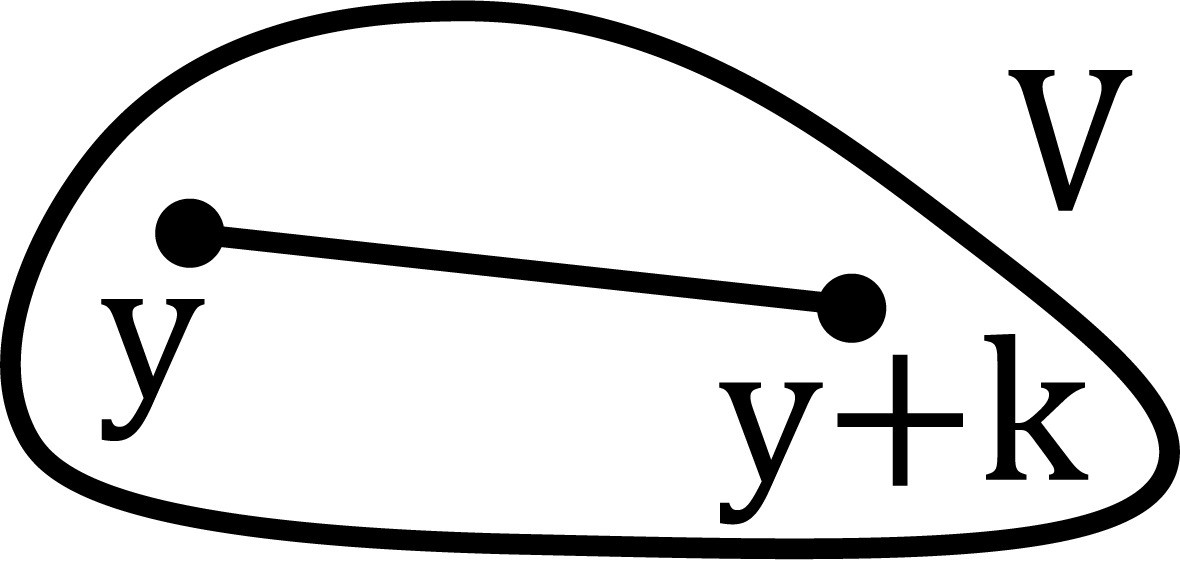
\includegraphics[width = 3cm]{pics/6_4}}
			\end{figure}
			\[y = f(x) \qq x = g(y)\]
			\[y + k = f(x + h) \q x + h = g(y + k)\]
			Докажем непр. на $V$:
			\[\Abs{\us{=h}{g(y + k) - g(y)}} = \Abs{h} \us{3\ (2b)}{\os{\text{по лемме}}{\leq}} \frac{1}{2\lambda}
				\Abs{\us{=f(x+h) - f(x)}{k}} \Ra g \text{ --- непр.}\]
			\[d_x f = A\]
			\[k = f(x + h) - f(x) = Ah + \alpha(h) \Abs{h} \q h \to 0\]
			\[A^{-1}k = h + A^{-1} (\alpha(h) \Abs{h})\]
			\[g(y + k) - g(y) - A^{-1}k = -A^{-1}(\alpha(h) \Abs{h}) \]
			\[\Abs{A^{-1}(\alpha(h) \Abs{h}) } \leq \Abs{A^{-1}} \cdot \abs{\us{< \E}{\alpha}} \Abs{h} \leq \]
			\[\leq \mathcal{E} \Abs{A^{-1}} \abs{h} \leq \mathcal{E} \Abs{A^{-1}} \frac{1}{2 \lambda}
				\Abs{k}\]
			\[\text{Т. о.}\q \lim_{k \to 0} \frac{\Abs{A^{-1}(\alpha \Abs{h}) }}{\Abs{k}} = 0\]
			\[f^{-1} \text{ --- непр. диф.? } \RLA \text{дифференциал --- непр., т.е.:}\]
			\[g = f^{-1} : V \to U_a, \q d_g : V \to \L (\R^n, \R^{2n} ) \q d_g \in C(V)\]
			\[\forall y \in V \q y \us{\text{непр.?}}{\to } d_{y} g \]
			\item $d_y g = \left(d_{g(y)} f \right)^{-1} \qq f \circ g = id \qq (f \circ g)(y) = y$
			\[d_{g(y)} f \cdot d_y g = E_n\q y \to d_y g\]
			\[y \to g(y) \to d_{g(y)} f \to (d_{g(y)} f )^{-1}  \]
			\[\text{Т.е. } y \to d_y g \text{ --- композиция трех непр. отображений}\]
		\end{enumerate}
	\end{proof}
\end{document}
